\subsubsection{Parsing}
Con \textit{Abstract Syntax Tree} (AST) si intende una struttura dati ad albero che 
rappresenta un'espressione, uno statement o una definizione 
di una variabile in un linguaggio di programmazione. L'AST è in corrispondenza 
biunivoca con il codice sorgente, e viene utilizzato
per rappresentare il codice sorgente in una forma più adatta per l'analisi 
e la manipolazione da parte del compilatore. \\

L'atto di trasformare una collezione ordinata di token in un AST \textbf{è chiamato \textit{parsing}}.

\begin{figure}[H]
    \centering
        \begin{tikzpicture}[
            node distance=1.5cm,
            elem/.style={
                circle, 
                draw=black, 
                thick, 
                text centered, 
                minimum height=2cm,
                minimum width=2cm
            },
            arrow/.style={
                ->, 
                thick
            }
        ]

            \node[elem] (plus) {+};
            \node[elem, below left=of plus] (x) {x};
            \node[elem, below right=of plus] (times) {*};
            \node[elem, below left=of times] (y) {y};
            \node[elem, below right=of times] (z) {z};

            \draw[arrow] (plus) -> (x);
            \draw[arrow] (plus) -> (times);
            \draw[arrow] (times) -> (y);
            \draw[arrow] (times) -> (z);
        \end{tikzpicture}
    \caption{Esempio di generico AST per un'espressione aritmetica "x + y * z"} 
\end{figure}
\newpage

In pratica, il compilatore Basalt utilizza internamente AST simili al seguente. Tale albero è 
ben più strutturato in quanto ogni nodo rappresenta un'entità del linguaggio ben precisa.

\begin{figure}[H]
    \centering
        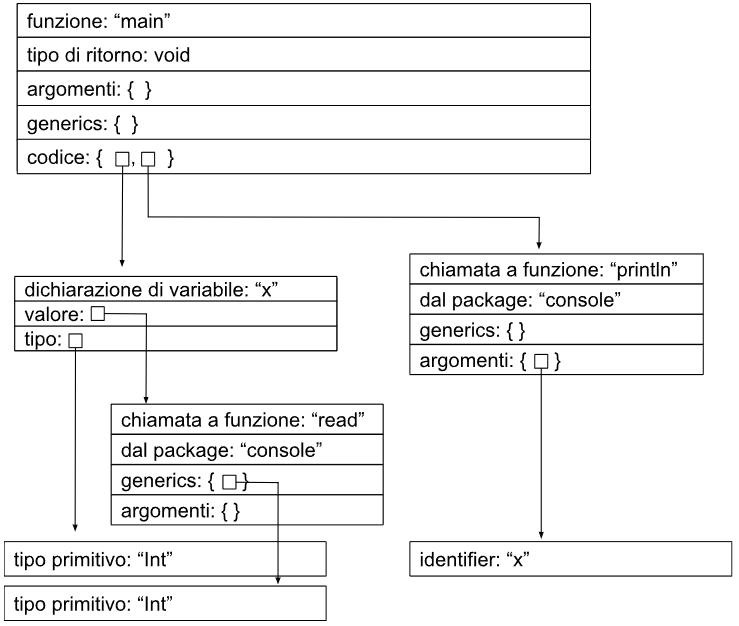
\includegraphics[width=1\textwidth]{../../Assets/BasaltAST.png}
    \caption{\centering Esempio di AST per una funzione main che legge da riga di comando un numero intero e lo stampa subito dopo} 
\end{figure}

Nei capitoli successivi sarà reso conto di come sia stato implementato il parsing in Basalt in dettaglio. Per completezza, si riporta che 
Esistono due principali famiglie di algoritmi di parsing: I parser \textit{LL} e i parser \textit{LR}. Tali parser differiscono per il modo in cui
essi costruiscono l'AST. I parser LL costruiscono l'AST scansionando i token da sinistra a destra e costruendo il sottoalbero sinistro completamente 
prima di passare al token seguente (leftmost-derivation). I parser LR, invece, seppur scansionano i token da sinistra a destra, costruiscono 
l'AST modificando e rifinendo il sottoalbero destro man mano che scoprono nuovi token (rightmost-derivation). \\
